\documentclass[11pt]{article}
\usepackage{geometry}                % See geometry.pdf to learn the layout options. There are lots.
\geometry{letterpaper}                   % ... or a4paper or a5paper or ... 
%\geometry{landscape}                % Activate for for rotated page geometry
%\usepackage[parfill]{parskip}    % Activate to begin paragraphs with an empty line rather than an indent
\usepackage{graphicx}
\usepackage{amssymb}
\usepackage{epstopdf}
\usepackage[usenames,dvipsnames]{color}
\usepackage{hyperref}
\usepackage{url}
\hypersetup{colorlinks=true}
%\DeclareGraphicsRule{.tif}{png}{.png}{`convert #1 `dirname #1`/`basename #1 .tif`.png}
\renewcommand\familydefault{\sfdefault}
\newcommand{\todo}[1]{{\bf\textcolor{red}{TODO: #1}}}
\setlength{\topmargin}{0cm}
\setlength{\headheight}{0cm}
\setlength{\headsep}{1cm}
\setlength{\textheight}{7.7in}
\setlength{\textwidth}{6.5in}
\setlength{\oddsidemargin}{0cm}
\setlength{\evensidemargin}{0cm}
\setlength{\parindent}{0.25cm}
\setlength{\parskip}{0.1cm}

\usepackage{fancyhdr,graphicx,lastpage}% http://ctan.org/pkg/{fancyhdr,graphicx,lastpage}
\fancypagestyle{plain}{
  \fancyhf{}% Clear header/footer
  \fancyhead[L]{CSCI-GA.2270-001 - Computer Graphics - Fall 17 }% Right header
  \fancyhead[R]{
\includegraphics[height=20pt]{nyu.pdf}}% Right header
  \fancyfoot[L]{Daniele Panozzo \\  \today}% Left footer
  \fancyfoot[R]{\thepage}% Right footer
}
\pagestyle{plain}% Set page style to plain.

\begin{document}

\hspace{50pt}

\begin{center}

{\Huge \textbf{Assignment 2: Rasterization}}\\
\vspace{10pt}
Handout date: 10/16/2017\\
Submission deadline: 11/5/2017,  23:59 EST\\
Demo date: TBA
\end{center}
%\vspace{0.5cm}

\noindent This homework accounts for 17.5\% of your final grade. 

\section*{Goal of this exercise}
In this exercise you will implement a 2D editor for vector graphics. The editor will allow to draw simple shapes interactively.

\subsection*{Eigen}
In all exercises you will need to do operations with vectors and matrices. To simplify the code, you will use \href{http://eigen.tuxfamily.org/}{\texttt{Eigen}}. 
Have a look at the \href{http://eigen.tuxfamily.org/dox/GettingStarted.html}{``Getting Started"} page of \texttt{Eigen} as well as the \href{http://eigen.tuxfamily.org/dox/group__QuickRefPage.html}{Quick Reference} page to acquaintain yourselves with the basic matrix operations supported. 

\subsection*{OpenGL}
In all exercises you will use OpenGL 3.3 with GLSL version 150.

\subsection*{Submission}

\begin{enumerate}
\item Follow the link sent by assistant to accept assignment and create repository.
\item Modify the code following the assignment instructions
\item Set up Travis-ci badge.
\item Add a report in pdf format that contains what you did with a screenshot for each task
\item Commit and push the code into the repository before the deadline.
\end{enumerate}


\section{Mandatory Tasks}
For each tasks below, add at least one image in the readme demonstrating the results. The code that you used for all tasks should be provided.

\subsection{Triangle Soup Editor}

Implement an interactive application that allows to add, edit, and delete triangles. The following operations should be supported:
\begin{itemize}
	\item The key 'i' will enable triangle insertion mode. When this mode is enabled, every triple of subsequent mouse clicks will create a triangle connecting the three locations where the mouse has been pressed. The first click will create the starting point of the segment, which will be immediately visualized. As the mouse is moved, a preview of a segment will appear. After the second mouse click, a preview of the triangle will appear. After the third click, the current preview will transform into the final triangle. 
\end{itemize}
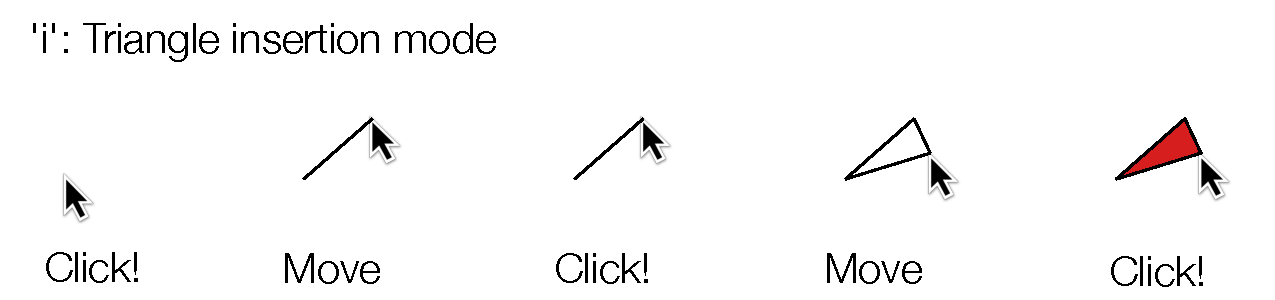
\includegraphics[width=1\textwidth]{i.pdf}
\begin{itemize}
	\item The key 'o' will enable triangle translation mode. Each mouse click will selected the triangle below the cursor (which will be highlighted), and every movement of the mouse (while keeping the button pressed) will result in a corresponding translation of the triangle. Note that the triangle should move on screen by the same amount as the cursor.
\end{itemize}
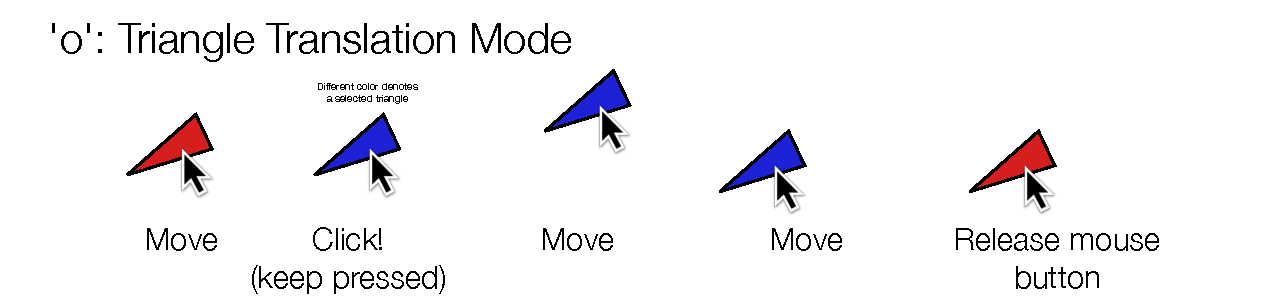
\includegraphics[width=1\textwidth]{o.pdf}
\begin{itemize}
	\item The key 'p' will enable delete mode. When the mouse is pressed, the triangle below the cursor is deleted.

\end{itemize}
\subsection{Rotation/Scale}

When triangle translation mode is enabled, keep the current primitive selected after the mouse is released. If a primitive is selected and you press the keys 'h' and 'j', the triangle will rotate by 10 degree clockwise or counter-clockwise, respectively. The rotations should be done around its barycenter, i.e. the barycenter of the triangle should not change. When the keys 'k' or 'l' are pressed, the primitive should be scaled up or down by 25\%. Similarly to before, the barycenter of the triangle should not move due to the scaling. For this task, you can directly edit the position of the vertices of the triangles on the CPU side, and re-upload them to the GPU after every change. If you do it directly in the vertex shader, you can gain additional points (see Task \ref{sec:shader})

\subsection{Colors}

Add the possibility to paint the color of each vertex in the scene. Color mode is enabled by the key 'c'. In this mode, every mouse click will select the vertex closer to the current mouse position. After a vertex is selected, pressing a key from '1' to '9' will change its color (the colors that you use are not important, you can pick whatever colors you like). The color should be interpolated linearly inside the triangles.

\subsection{View Control}

Add to the application the capability of changing the camera. The following actions should be supported:
\begin{itemize}
	\item '+' should increase the zoom by 20\% zooming in in the center of the screen
	\item '-' should decrease the zoom by 20\% zooming out in the center of the screen
	\item 'w', 'a', 's', and 'd' should pan the view by 20\% of the visible part of the scene, i.e. translate the entire scene, respectively down, right, up and left by 20\% of the window size.
\end{itemize}

This should NOT be implemented by changing the coordinates of the objects in the scene. You must add a view matrix to the vertex shader (as a uniform) that is transforming the position of the vertices of the triangles before they are rendered. Note that you will also have to transform the screen coordinates using the inverse of the view matrix, to ensure that the user interaction will adapt to the current view.
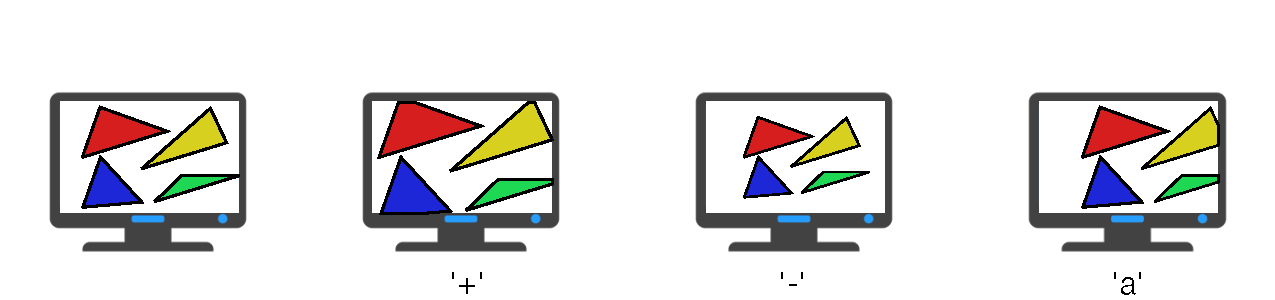
\includegraphics[width=1\textwidth]{view.pdf}

\subsection{Add keyframing}

Add the possibility to keyframe one property of an object (size,  position, or rotation) and create an animation using linear interpolation between the keyframes. You can use a timer to make the animation automatic, or you could move to the next frame at the press of a button.

\section*{Optional Tasks}

These tasks are optional. Each one of these tasks is worth 1.5\% of the final grade. The optional points are added to the points of the other exercises, but the total sum of points that you gain with exercises cannot be more than 80\%.

\subsection{Additional primitive}

Add a new mode that allows to add bezier curves and to move their control points.

\subsection{Export in SVG format}

Add the possibility to export the current drawing in SVG format \url{https://en.wikipedia.org/wiki/Scalable_Vector_Graphics}. The exported SVG should be compatible with \url{https://inkscape.org/}.

\subsection{Shader translation/scaling/rotation}
\label{sec:shader}
Upload every single triangle as a separate primitive in a separate VBO (or in a single VBO using offsets for drawing them one by one). For each primitive, upload to the GPU its model matrix (as a uniform) that transforms the triangle from its canonical position (defined at its creation) to the current position (obtained by combining translations, scaling and rotations). The transformation should be executed in the shader, and the content of the VBO storing the vertex positions never updated.

%\bibliographystyle{plain}
%\bibliography{bib.bib}
\end{document}  